\subsection{Konfigurasi Deployment Kluster Sistem Backend}

\subsubsection{Sistem Pengawasan}

\begin{figure}[htbp]
    \centering
    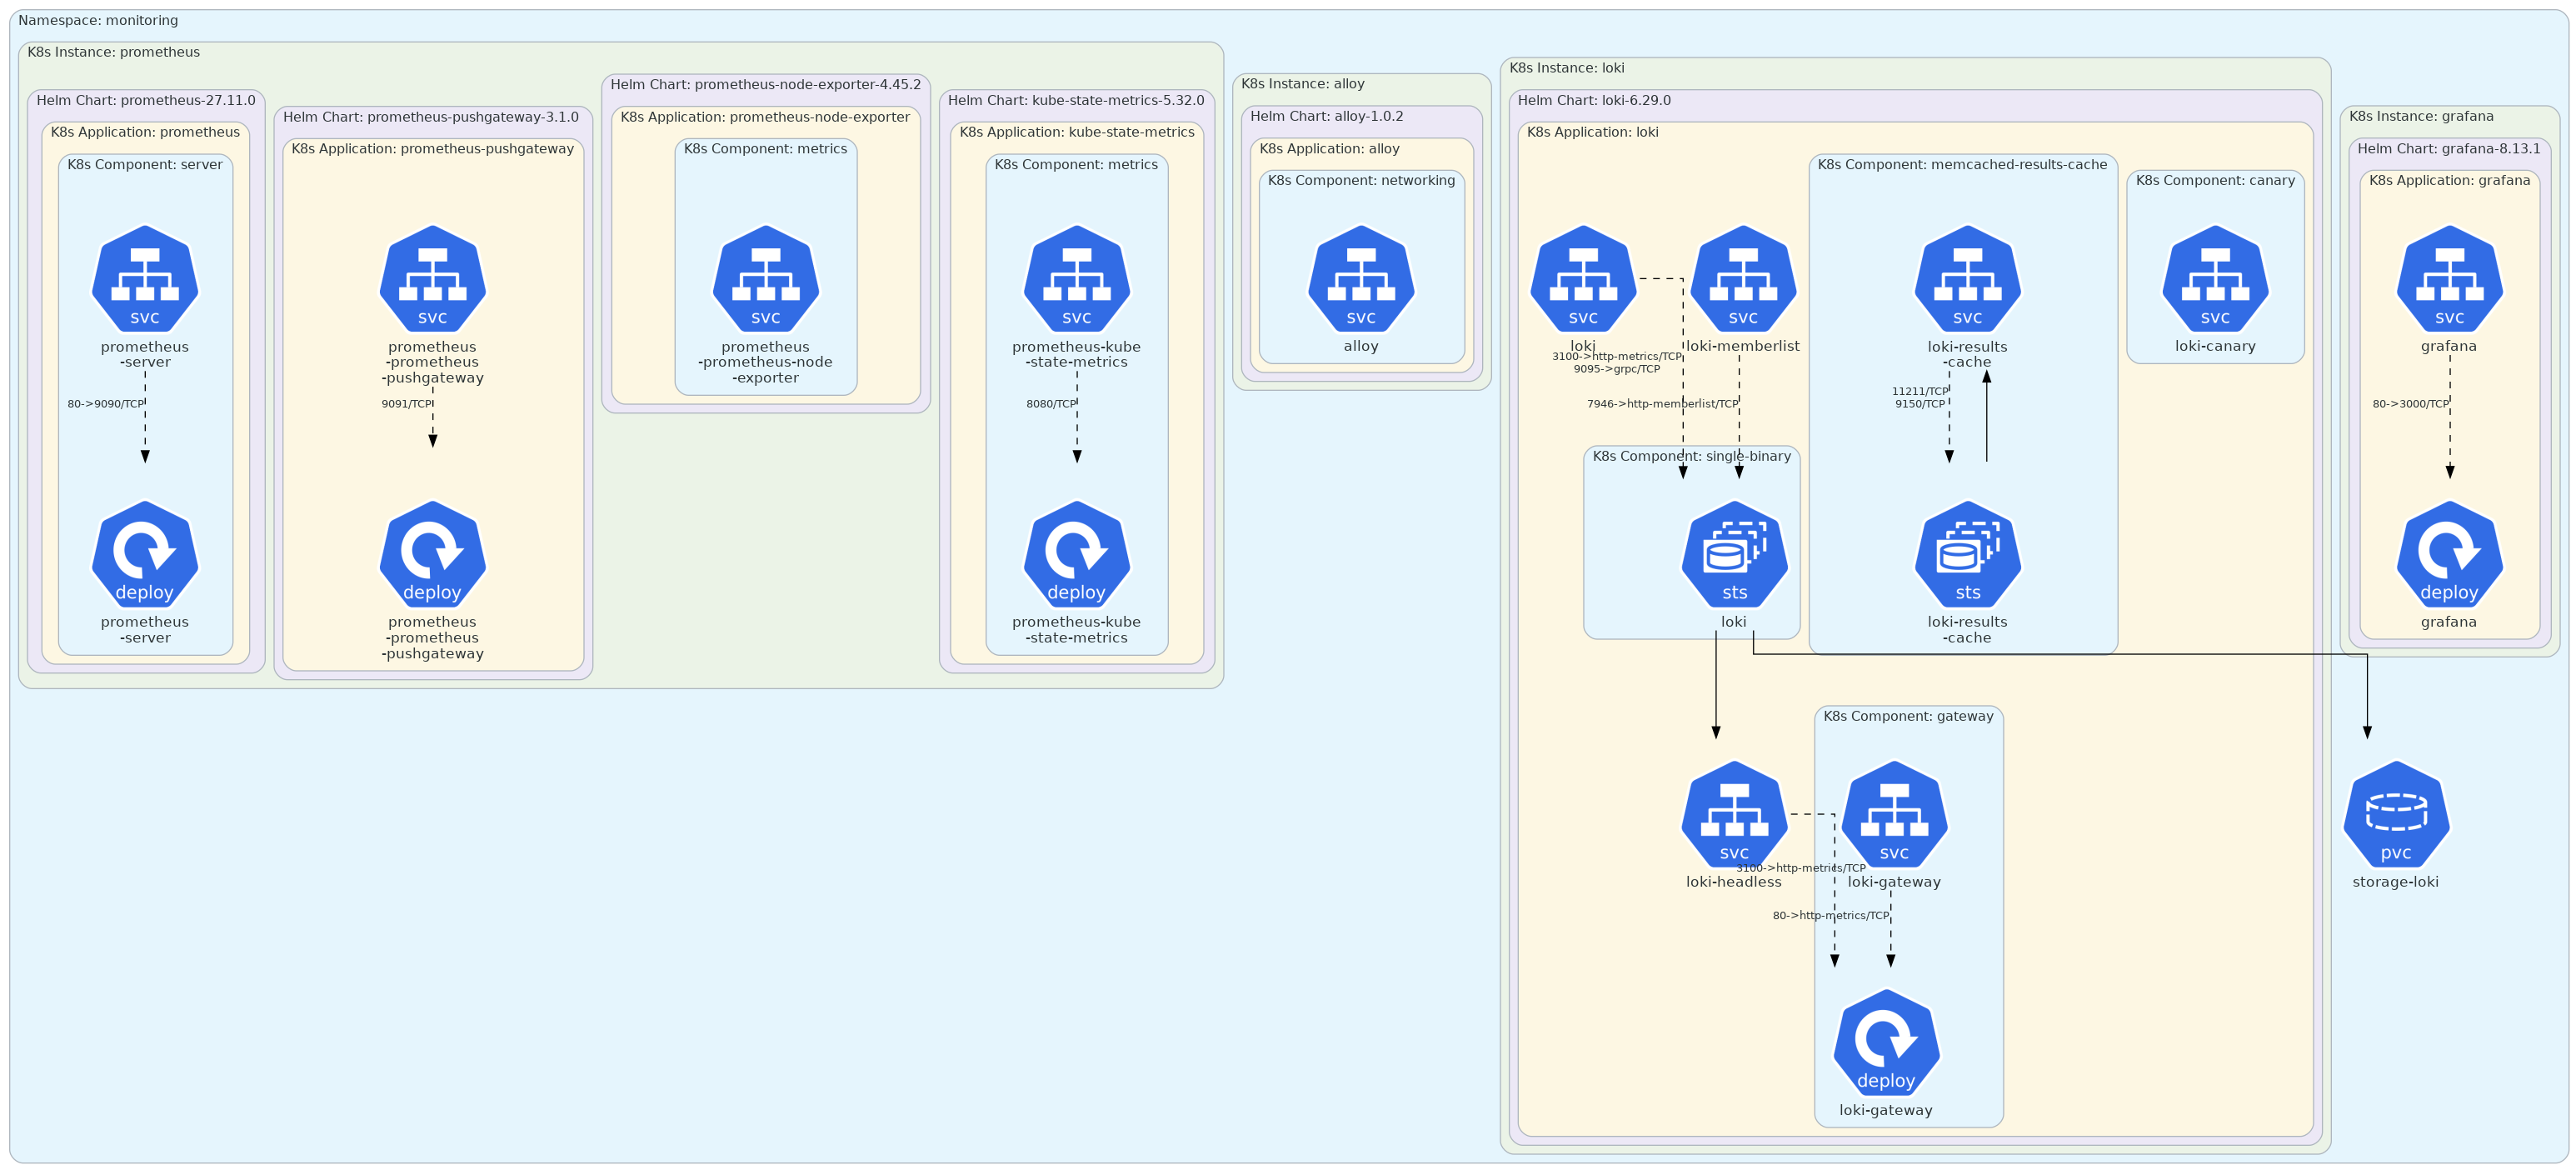
\includegraphics[width=1\textwidth]{resources/chapter-4/monitoring.png}
    \caption{Deployment Sistem Monitoring}
    \label{fig:deployment-monitoring}
\end{figure}

Sebagaimana dibahas pada bagian sebelumnya, komponen utama dari sistem pengawasan ini terdiri atas Grafana Alloy, Grafana Loki, Grafana Dashbaord, dan Prometheus. Meskipun begitu, terdapat beberapa service dan container tambahan yang merupakan konfigurasi default dari chart yang digunakan.

\pagebreak

\subsubsection{Nginx Ingress Controller}

\begin{figure}[htbp]
    \centering
    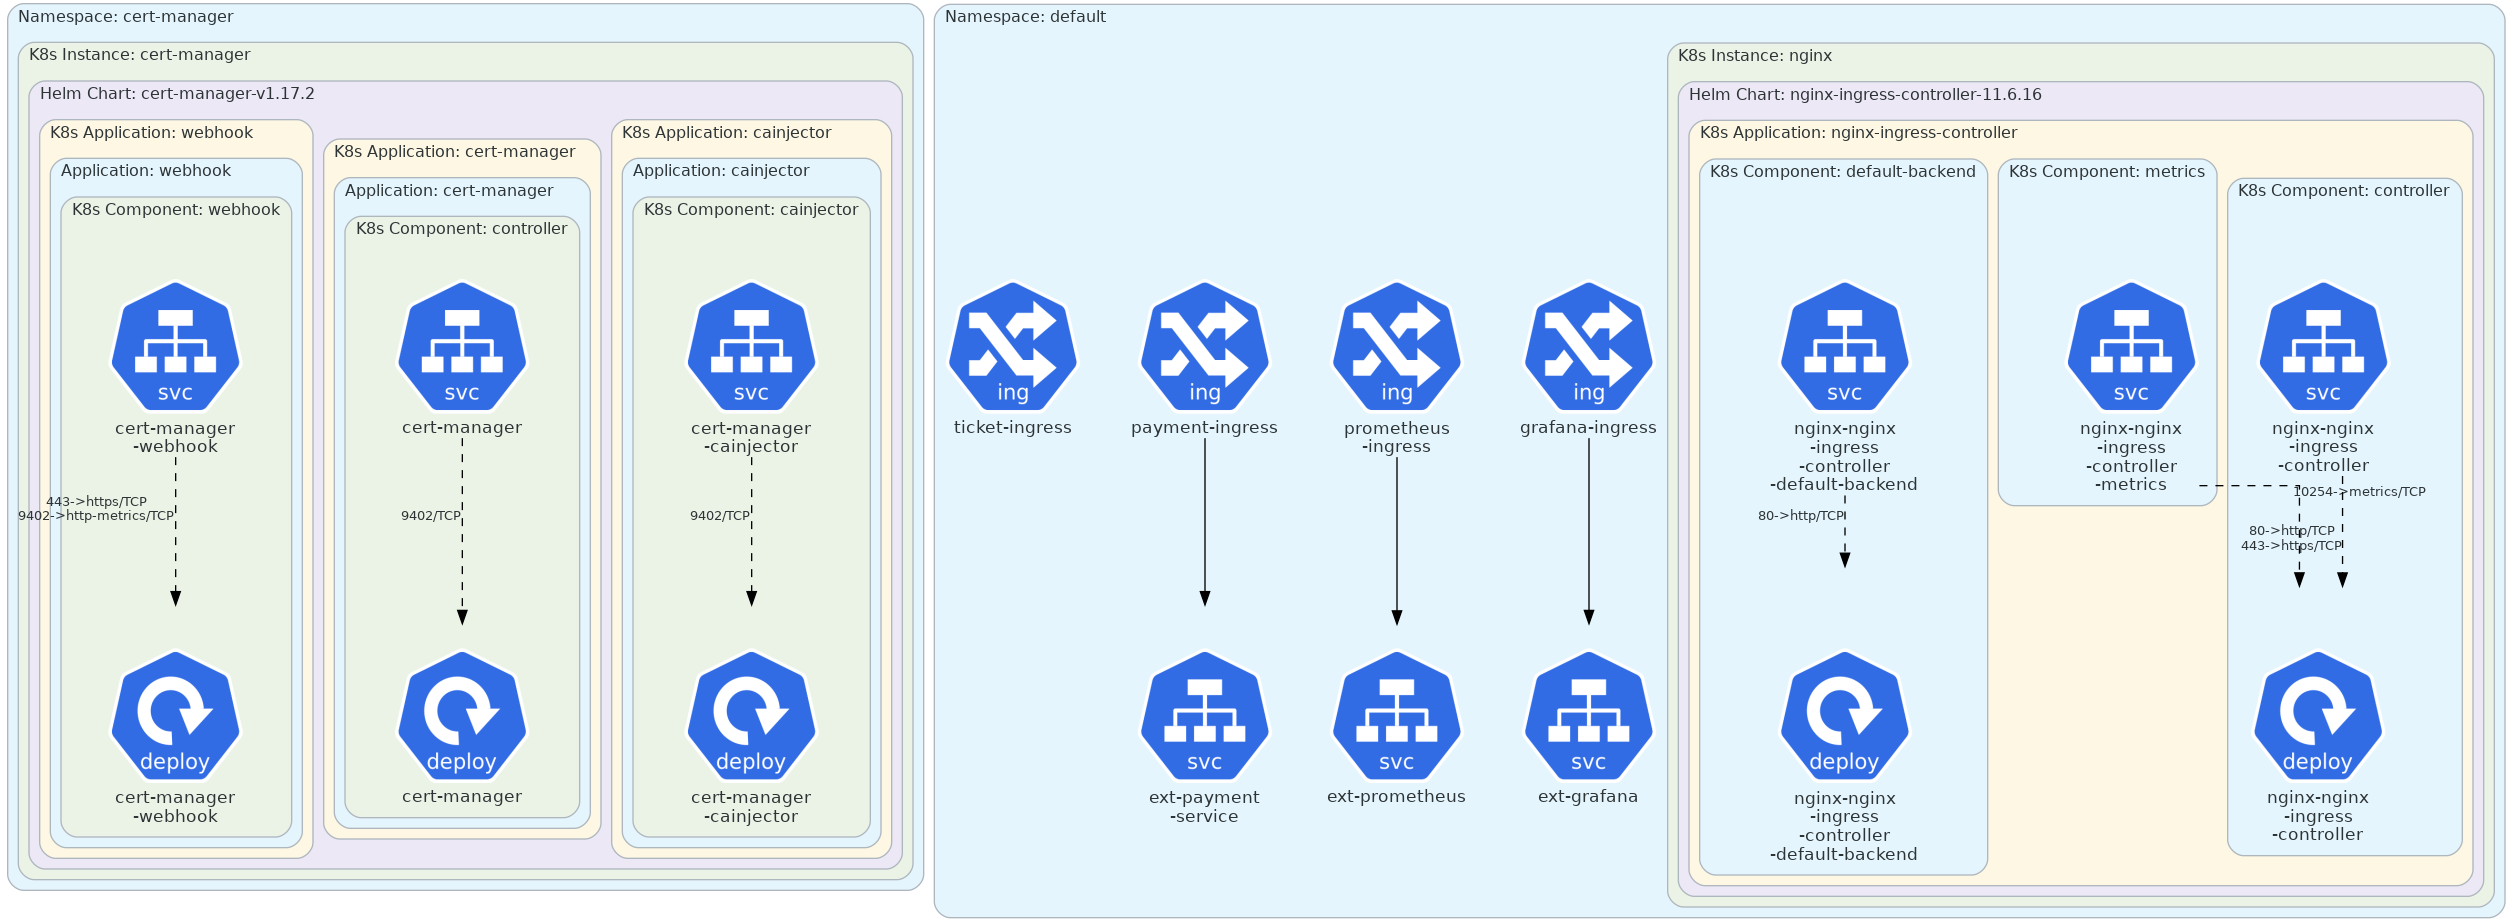
\includegraphics[width=1\textwidth]{resources/chapter-4/nginx.png}
    \caption{Deployment Nginx Ingress}
    \label{fig:deployment-nginx}
\end{figure}

Sistem ini terdiri atas cert-manager untuk menangani sertifikat SSL domain secara otomatis, deployment dan service Nginx Ingress Controller, serta beberapa ingress yang mengekspos layanan internal kubernetes ke dunia luar. Pada kluster ini terdapat empat layanan yang diekspos, yaitu layanan tiket, layanan pembayaran, dasbor prometheus, dan dasbor Grafna.

\pagebreak

\subsubsection{Layanan Pembayaran}

\begin{figure}[htbp]
    \centering
    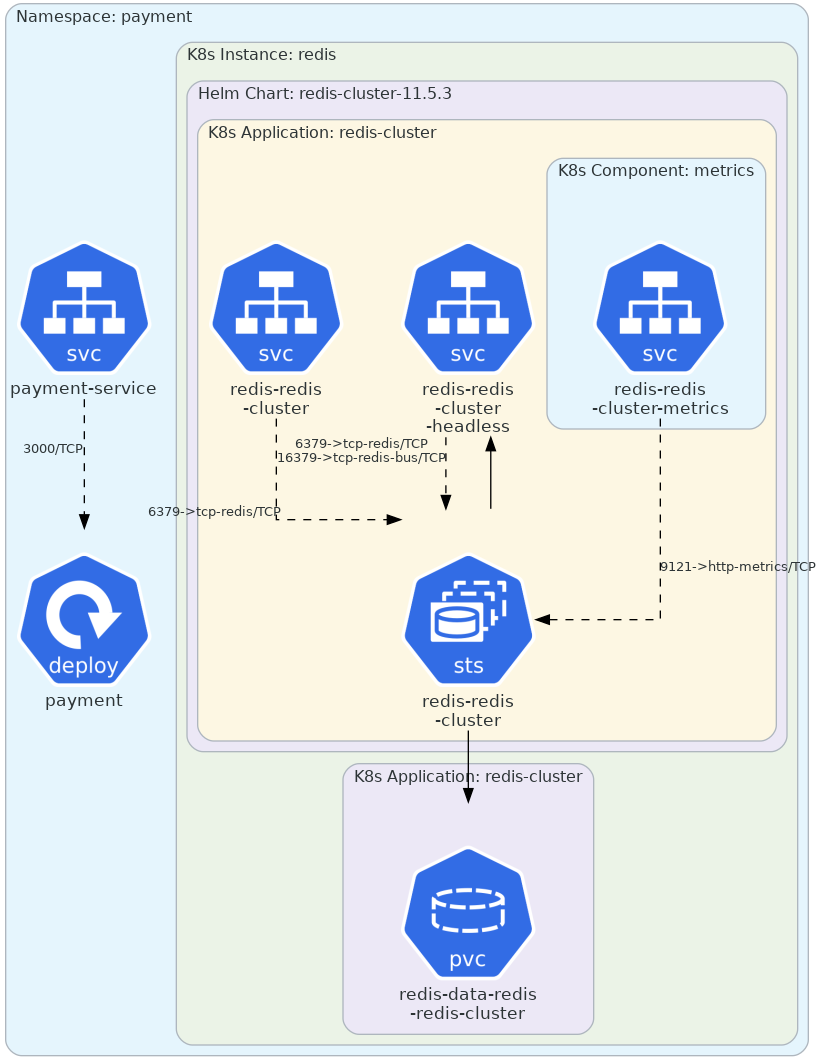
\includegraphics[width=0.8\textwidth]{resources/chapter-4/payment.png}
    \caption{Deployment Layanan Pembayaran}
    \label{fig:deployment-payment}
\end{figure}

Layanan pembayaran secara umum terdiri atas deployment payment, service payment, dan kluster Redis. Deployment payment terdiri atas dua container, yaitu payment service dan payment notifier.

\pagebreak

\subsubsection{Layanan Tiket varian tanpa \textit{Flow Control}}

\begin{figure}[htbp]
    \centering
    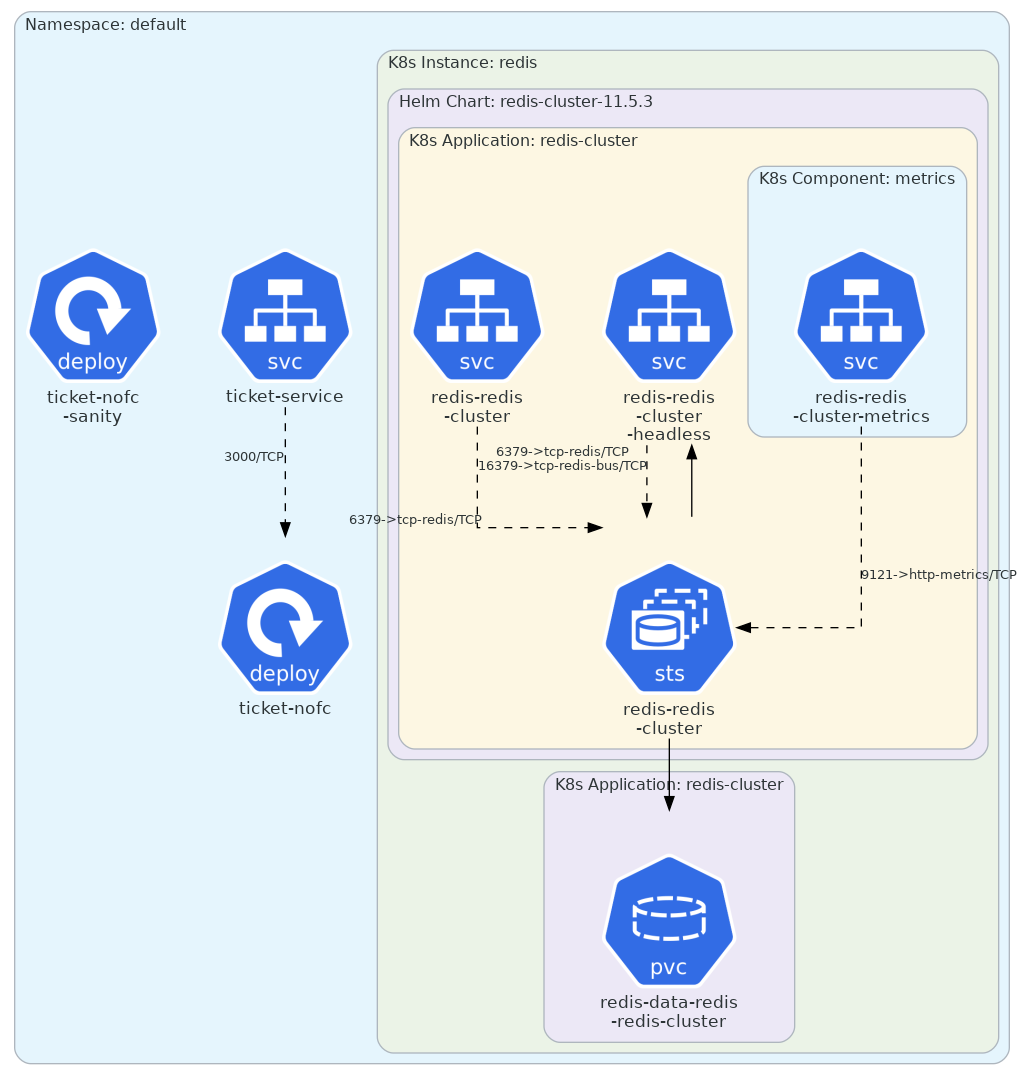
\includegraphics[width=1\textwidth]{resources/chapter-4/ticket-nofc.png}
    \caption{Deployment Layanan Ticket tanpa \textit{Flow Control}}
    \label{fig:deployment-ticket-nofc}
\end{figure}

Layanan tiket tanpa \textit{flow control} terdiri atas deployment ticket server, kluster redis, dan sanity check. Sistem ini juga terhubung dengan salah satu kluster basis data relasional yang ada melalui Pgbouncer.

\pagebreak

\subsubsection{Layanan Tiket varian dengan \textit{Flow Control}}

\begin{figure}[htbp]
    \centering
    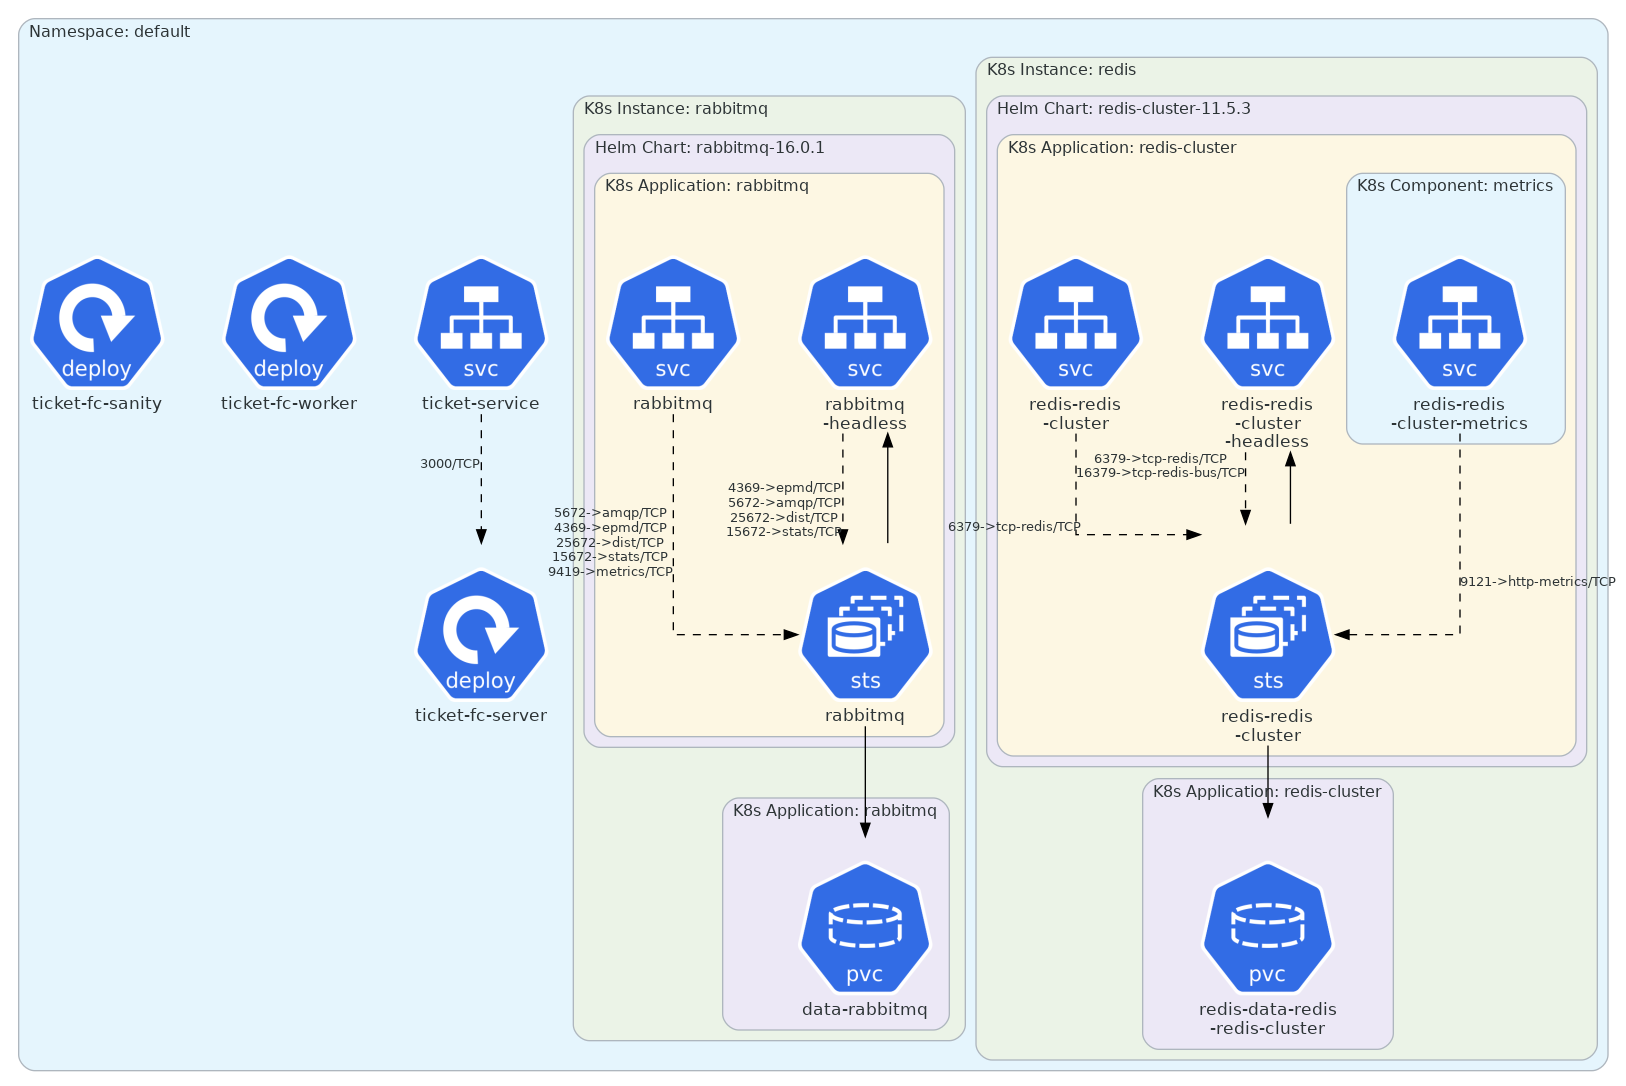
\includegraphics[width=1\textwidth]{resources/chapter-4/ticket-fc.png}
    \caption{Deployment Layanan Ticket dengan \textit{Flow Control}}
    \label{fig:deployment-ticket-fc}
\end{figure}

Layanan tiket dengan \textit{flow control} terdiri atas deployment ticket server, ticket-worker, kluster redis, rabbitmq, dan sanity check. Sistem ini juga terhubung dengan salah satu kluster basis data relasional yang ada melalui Pgbouncer.

\pagebreak

\subsubsection{Kluster PostgreSQL}

\begin{figure}[htbp]
    \centering
    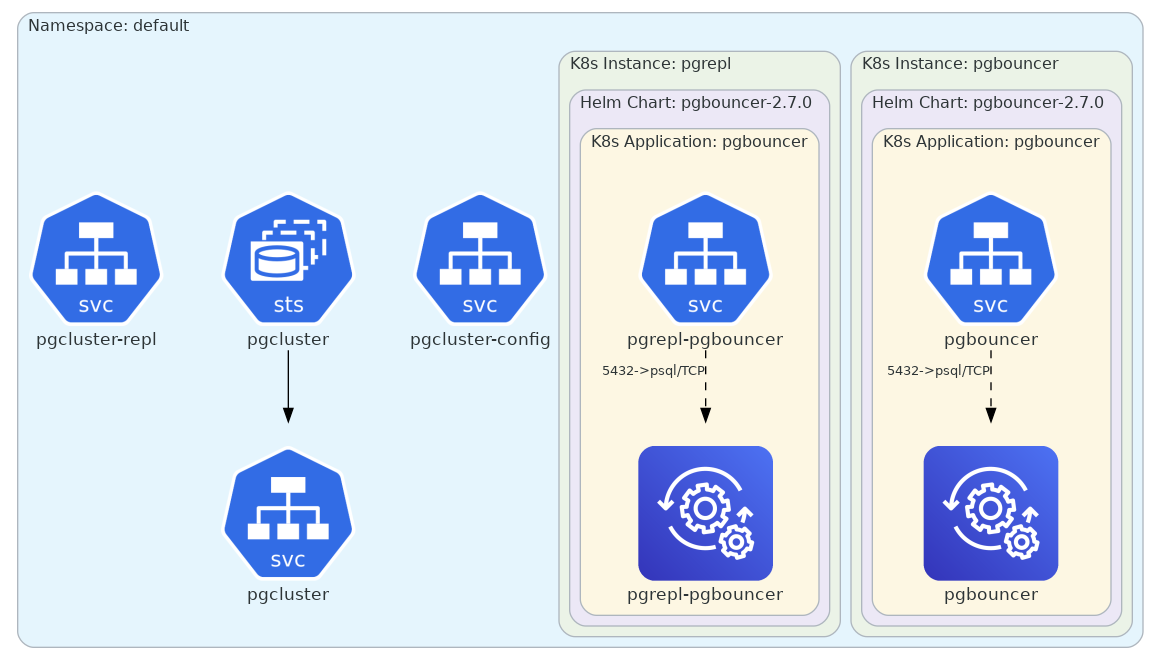
\includegraphics[width=1\textwidth]{resources/chapter-4/postgres.png}
    \caption{Deployment kluster PostgreSQL}
    \label{fig:deployment-postgres}
\end{figure}

Kluster PostgreSQL terdiri atas stateful set PostgreSQL yang akan terdiri atas satu primary dan satu replica. Selain itu, terdapat dua layanan pgbouncer. Satu untuk primary dan satu lagi untuk replica. Pemisahan ini dilakukan agar sistem tiket dapat terhubung dengan basis data melalui pgbouncer dengan multihost connection string sebagaimana didukung pada libpq. Keunggulan dari pendekatan ini adalah dengan tidak diperlukannya implementasi tambahan dari sisi sistem tiket.

\pagebreak

\subsubsection{Kluster CitusData}

\begin{figure}[htbp]
    \centering
    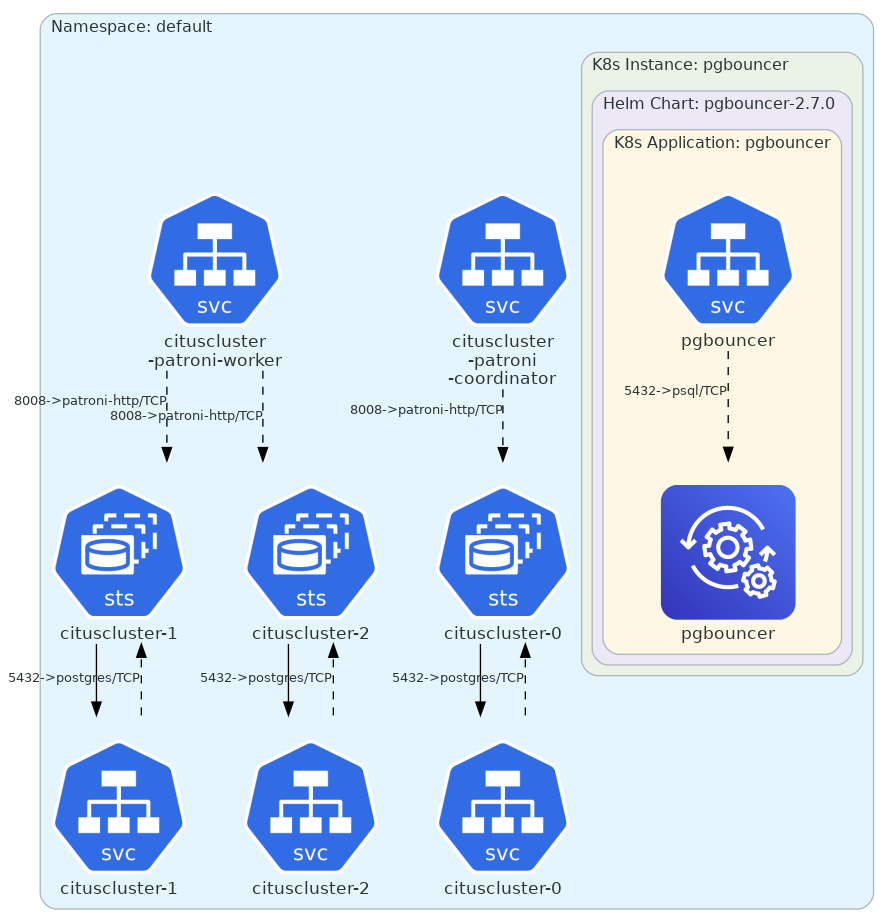
\includegraphics[width=1\textwidth]{resources/chapter-4/citusdata.png}
    \caption{Deployment kluster CitusData}
    \label{fig:deployment-citusdata}
\end{figure}

Kluster CitusData terdiri atas tiga stateful set CitusCluster. Cluster pertama merupakan koordinator dan sisanya merupakan worker. Terdapat Pgbouncer yang terhubung dengan koordinator. Sistem tiket terhubung langsung dengan Pgbouncer. Koneksi dengan worker dilakukan melalui koordinator.

\pagebreak

\subsubsection{Kluster YugabyteDB}

\begin{figure}[htbp]
    \centering
    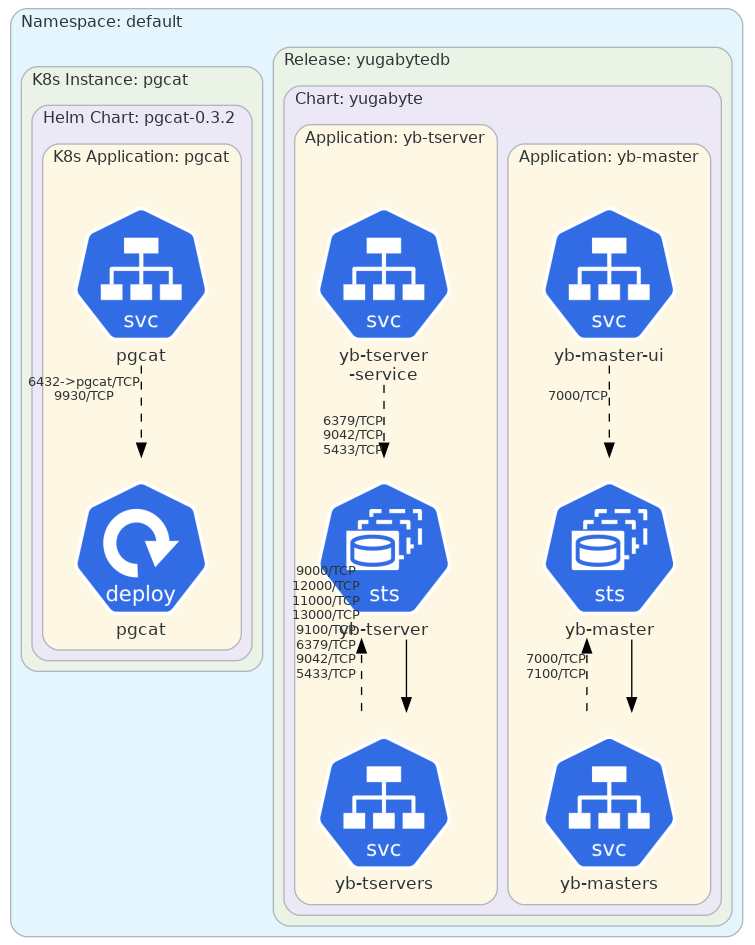
\includegraphics[width=1\textwidth]{resources/chapter-4/yugabyte.png}
    \caption{Deployment kluster YugabyteDB}
    \label{fig:deployment-yugabyte}
\end{figure}

Kluster YugabyteDB terdiri atas stateful set yugabyte master, stateful set yugabyte tablet server, dan pgbouncer. Pgbouncer terhubung dengan semua instance yugabyte master. Sistem tiket terhubung langsung dengan Pgbouncer. Koneksi dengan yugabyte master di-\textit{load balance} oleh Pgbouncer.

\pagebreak

\subsection{Konfigurasi Deployment Kluster Agen Penguji}

\subsubsection{Sistem Pengawasan}

\begin{figure}[htbp]
    \centering
    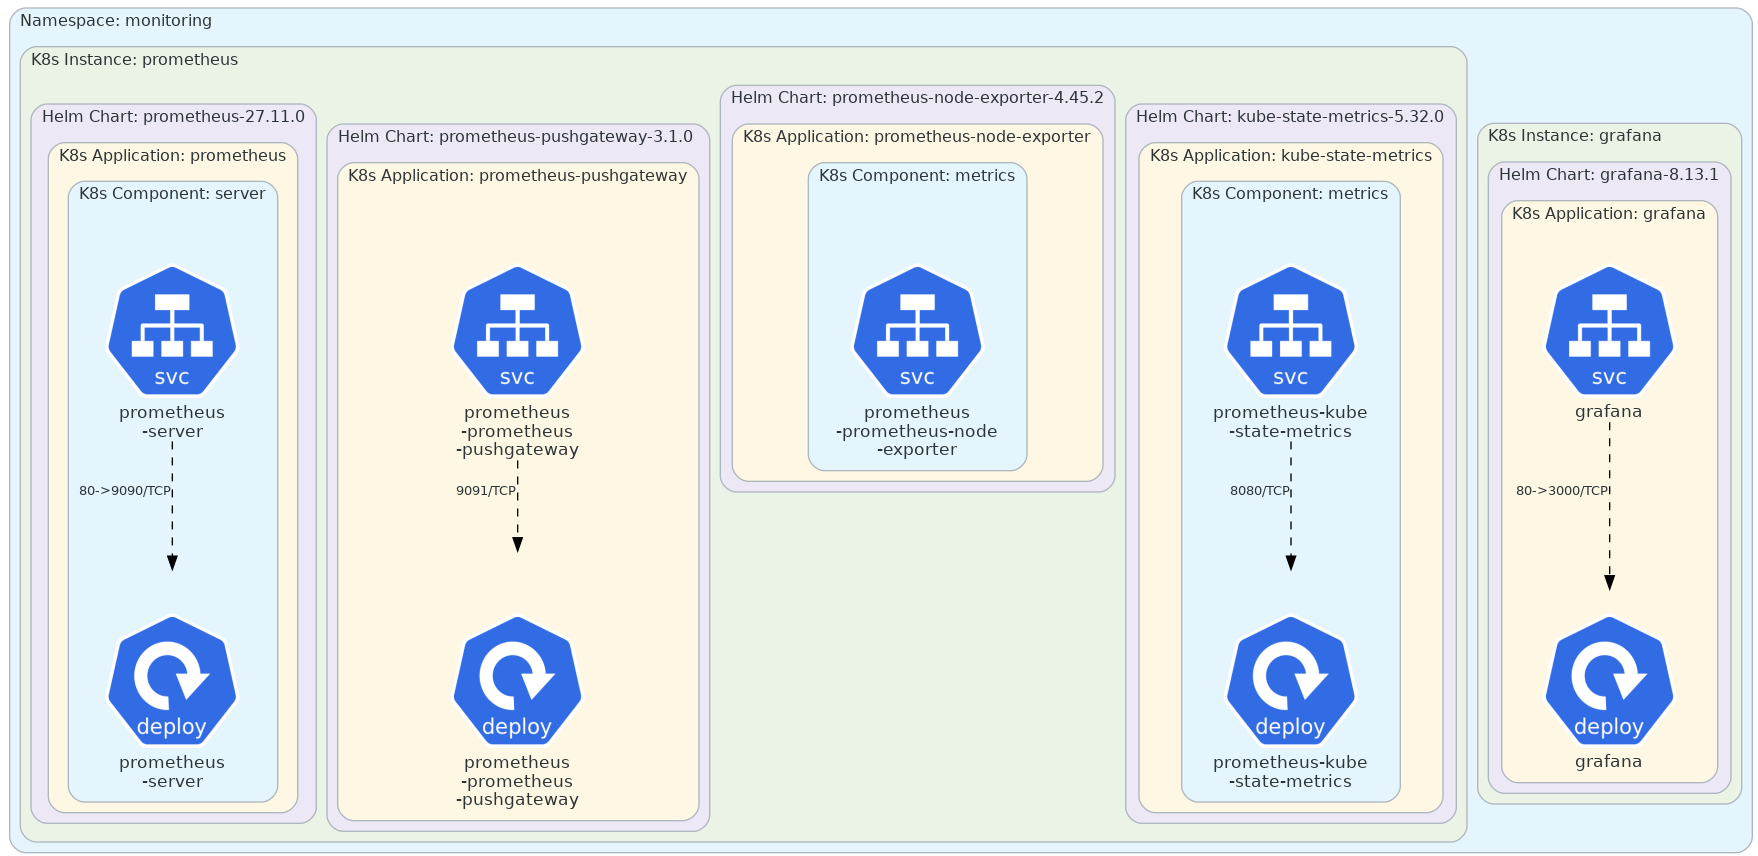
\includegraphics[width=1\textwidth]{resources/chapter-4/agent-monitoring.png}
    \caption{Deployment Sistem Monitoring}
    \label{fig:deployment-monitoring-agent}
\end{figure}

Sistem pengawasan pada agen penguji lebih sederhana dengan komponen hanya terdiri atas Grafana Dashboard dan Prometheus.

\pagebreak

\subsubsection{Nginx Ingress Controller}

\begin{figure}[htbp]
    \centering
    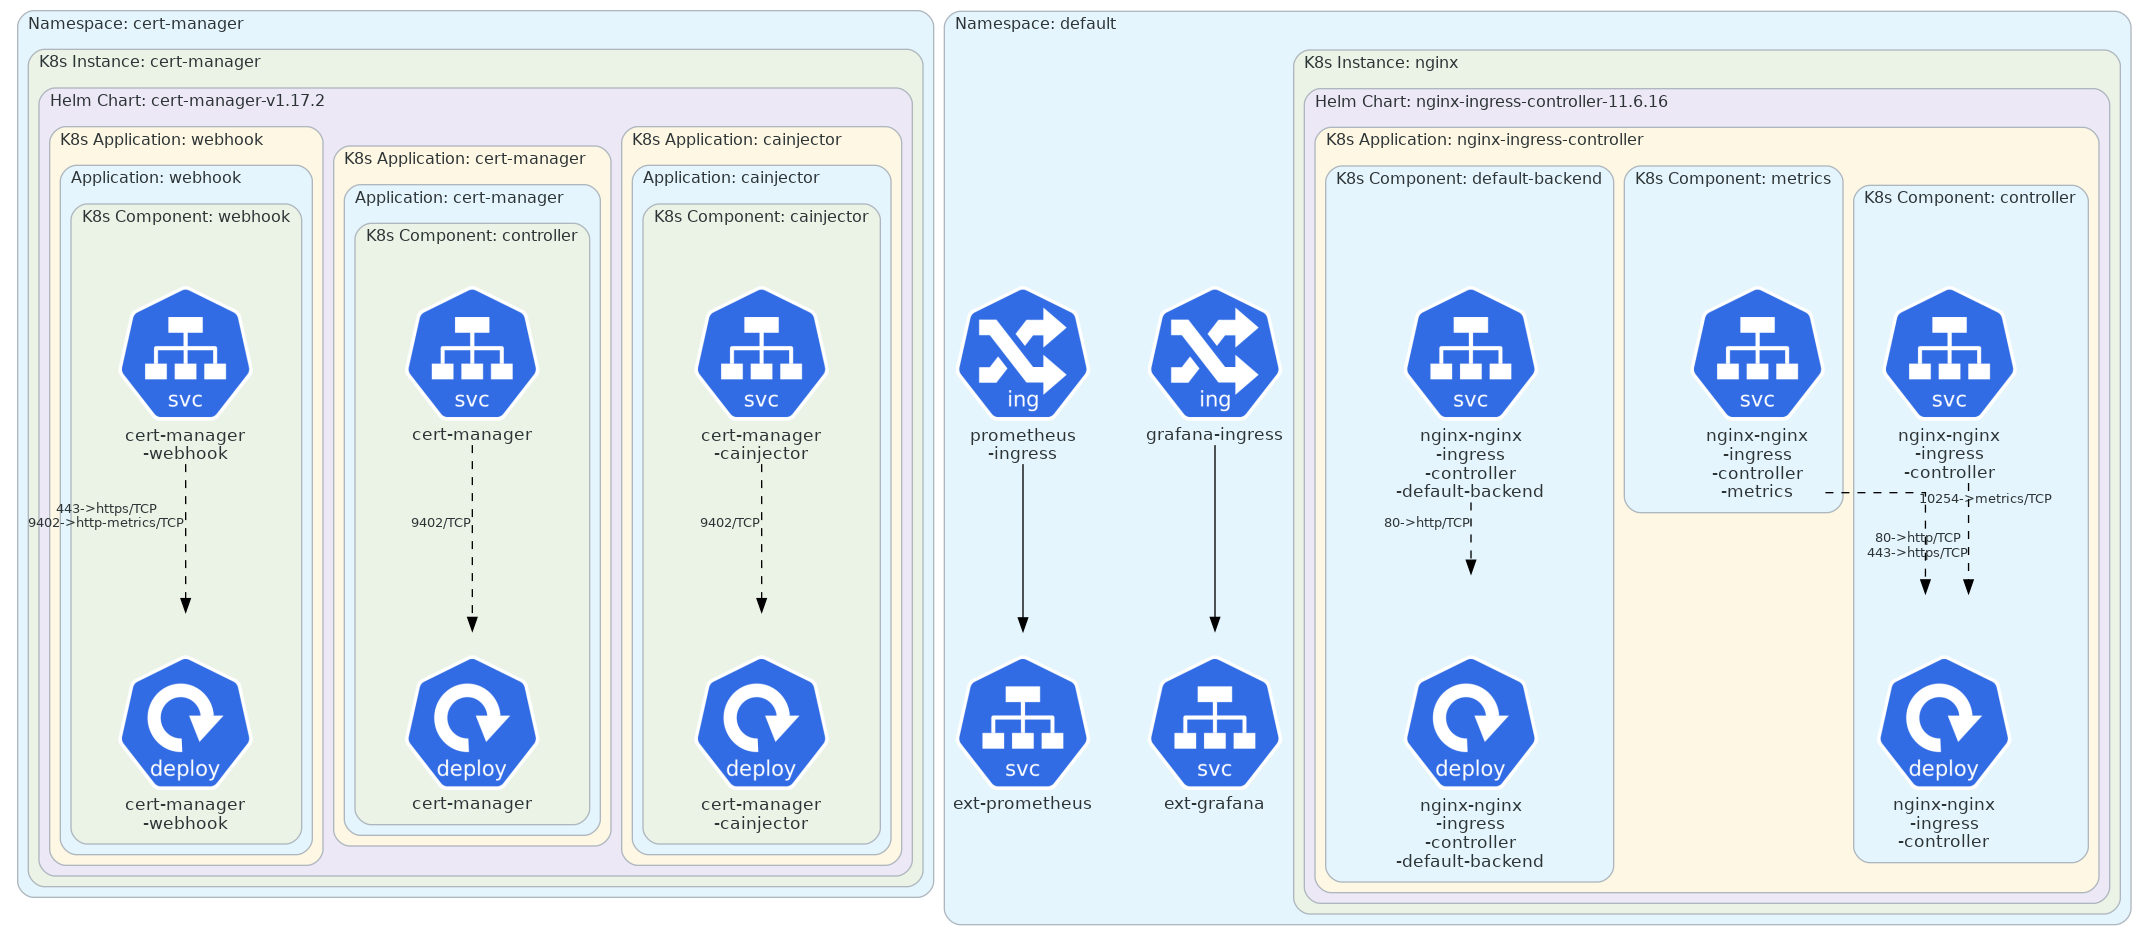
\includegraphics[width=1\textwidth]{resources/chapter-4/agent-nginx.png}
    \caption{Deployment Nginx Ingress}
    \label{fig:deployment-nginx-agent}
\end{figure}

Sistem ini terdiri atas cert-manager untuk menangani sertifikat SSL domain secara otomatis, deployment dan service Nginx Ingress Controller, serta beberapa ingress yang mengekspos layanan internal kubernetes ke dunia luar. Pada kluster ini terdapat dua layanan yang diekspos, yaitu dasbor prometheus dan dasbor Grafna.

\pagebreak

\subsubsection{K6 Operator}

\begin{figure}[htbp]
    \centering
    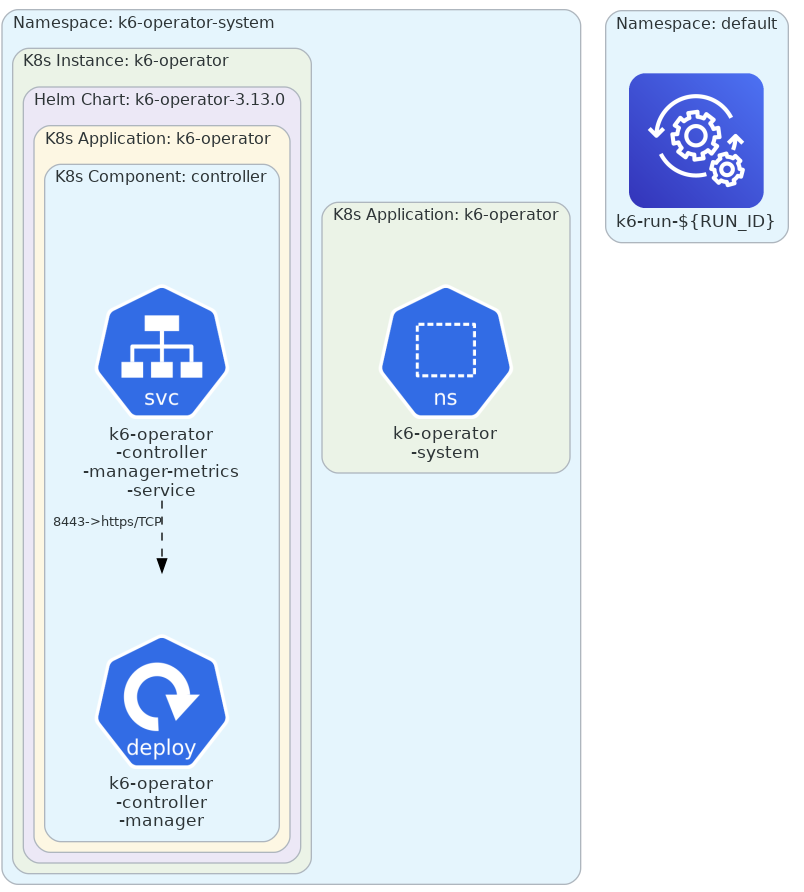
\includegraphics[width=1\textwidth]{resources/chapter-4/k6-operator.png}
    \caption{Deployment K6 Operator}
    \label{fig:deployment-k6-operator}
\end{figure}

K6 Operator merupakan komponen utama kluster penguji. Komponen ini mengatur inisiasi dan runtime script pengujian k6.

\pagebreak